\documentclass[12pt]{article}

\usepackage{lmodern}
\usepackage[T1]{fontenc}
\usepackage[utf8]{inputenc}
\usepackage[spanish, activeacute]{babel}
\usepackage{listings}
\usepackage{enumitem}
\usepackage{graphicx}
\usepackage{float}
\usepackage[hidelinks]{hyperref}
\usepackage{xcolor}

\definecolor{codegreen}{rgb}{0,0.6,0}
\definecolor{codegray}{rgb}{0.5,0.5,0.5}
\definecolor{codepurple}{rgb}{0.58,0,0.82}
\definecolor{backcolour}{rgb}{0.95,0.95,0.92}

\lstdefinestyle{mystyle}{
    backgroundcolor=\color{backcolour}, 
    commentstyle=\color{codegreen},
    keywordstyle=\color{magenta},
    numberstyle=\tiny\color{codegray},
    stringstyle=\color{codepurple},
    basicstyle=\ttfamily\footnotesize,
    breakatwhitespace=false,         
    breaklines=true,                 
    captionpos=b,                    
    keepspaces=true,                 
    numbers=left,                    
    numbersep=5pt,                  
    showspaces=false,                
    showstringspaces=false,
    showtabs=false,         
    tabsize=2
}

\lstset{style=mystyle}

\graphicspath {{ assets/images/ }}

\title{Práctica 02 - Fundamentos de NodeJS}
\author{ 
    Wilson Aguilar \\
    \textsc{Plataformas Web} 
}

\begin{document}

\maketitle

\section{Let vs Var}

En Javascript tenemos las palabras reservadas \lstinline{let} y \lstinline{var} que nos permiten la declaracion de una variable. La diferencia entre estas palabras radica en su alcance. 

Let se limita al scope de donde fue définida, mientras que var tiene un alcance global y puede ser llamado fuera del scope.

\begin{figure}[H]
	\centering
	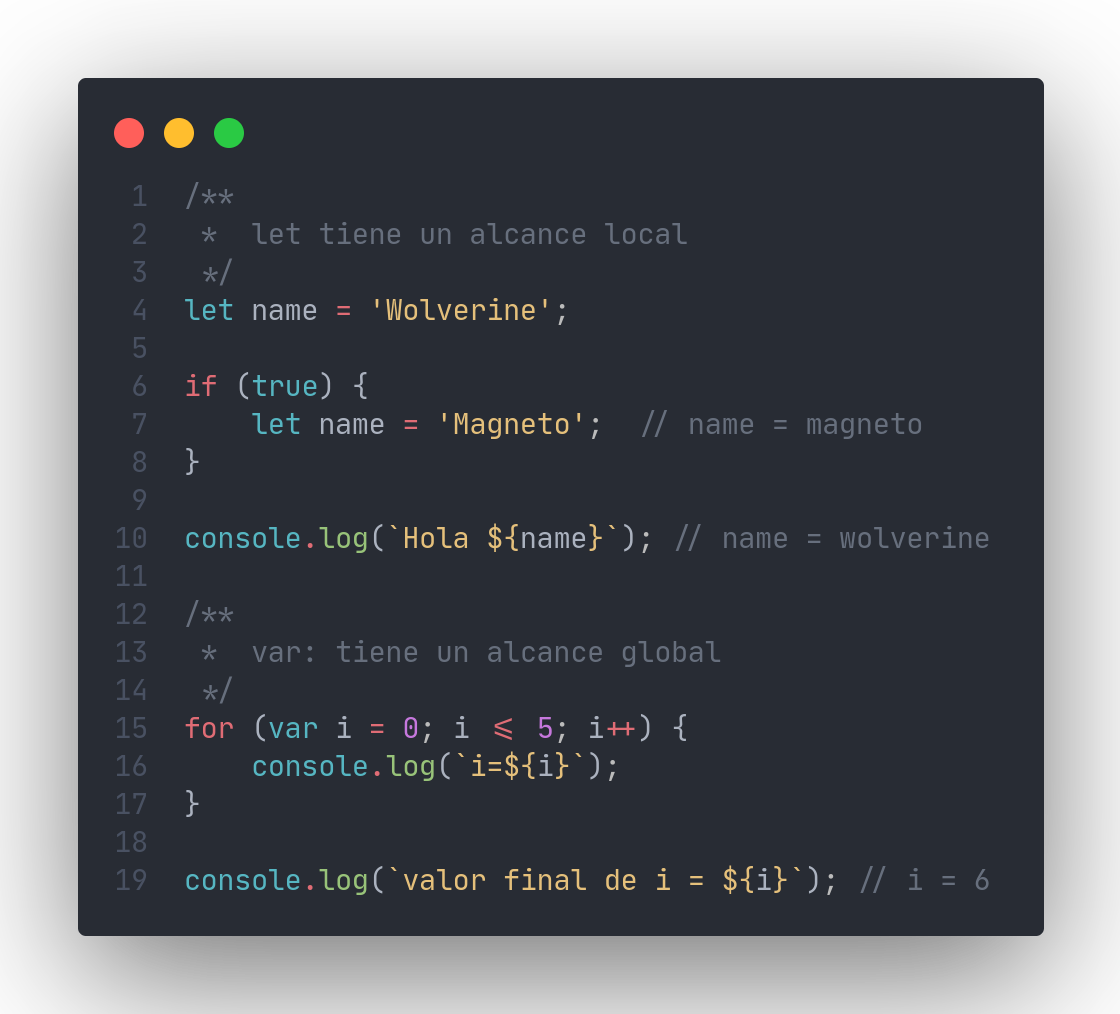
\includegraphics[scale=.23]{assets/images/let-var.png}
	\caption{Ejemplo de let y var}
\end{figure}

\section{Template literals}

Los template literals o plantillas de cadena es una nueva forma de definir una cadena, solo que en este caso podemos inyectar directamente una variable o funcion dentro de la cadena de texto.

\begin{figure}[H]
	\centering
	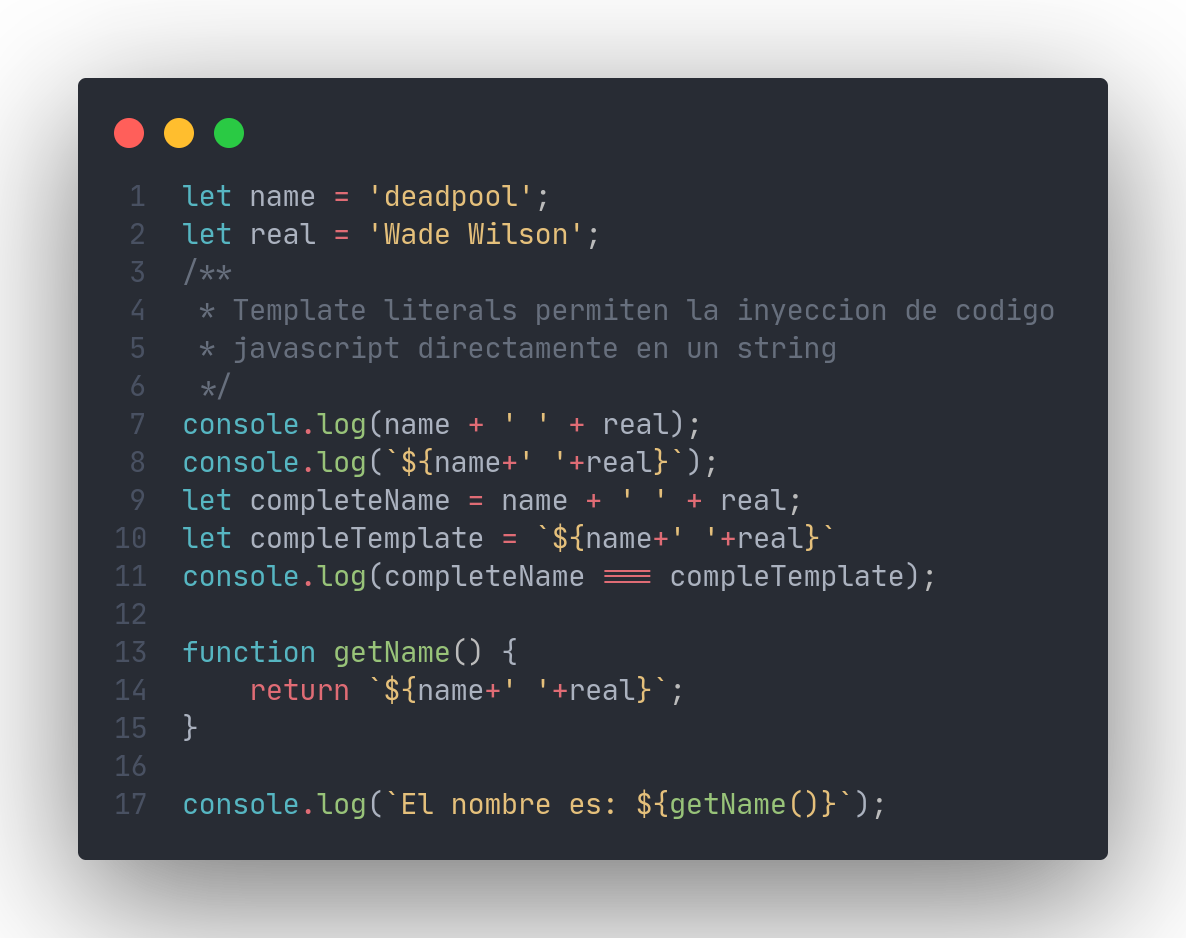
\includegraphics[scale=.3]{assets/images/template-literals.png}
	\caption{Ejemplo de template literals}
\end{figure}

Los template literals son muy usados en frameworks de Javascript enfocados al front-end. Lo utilizan para crear un fragmento o template de un componente de HTML y luego inyectan la variable que va a ser dinámica directamente en el string, lo que hace que el código sea mejor legible.



\newpage

\section{Destructuración}

La destrucutracion nos permite extraer variables que se encuentran dentro de un objeto. 

\begin{figure}[H]
	\centering
	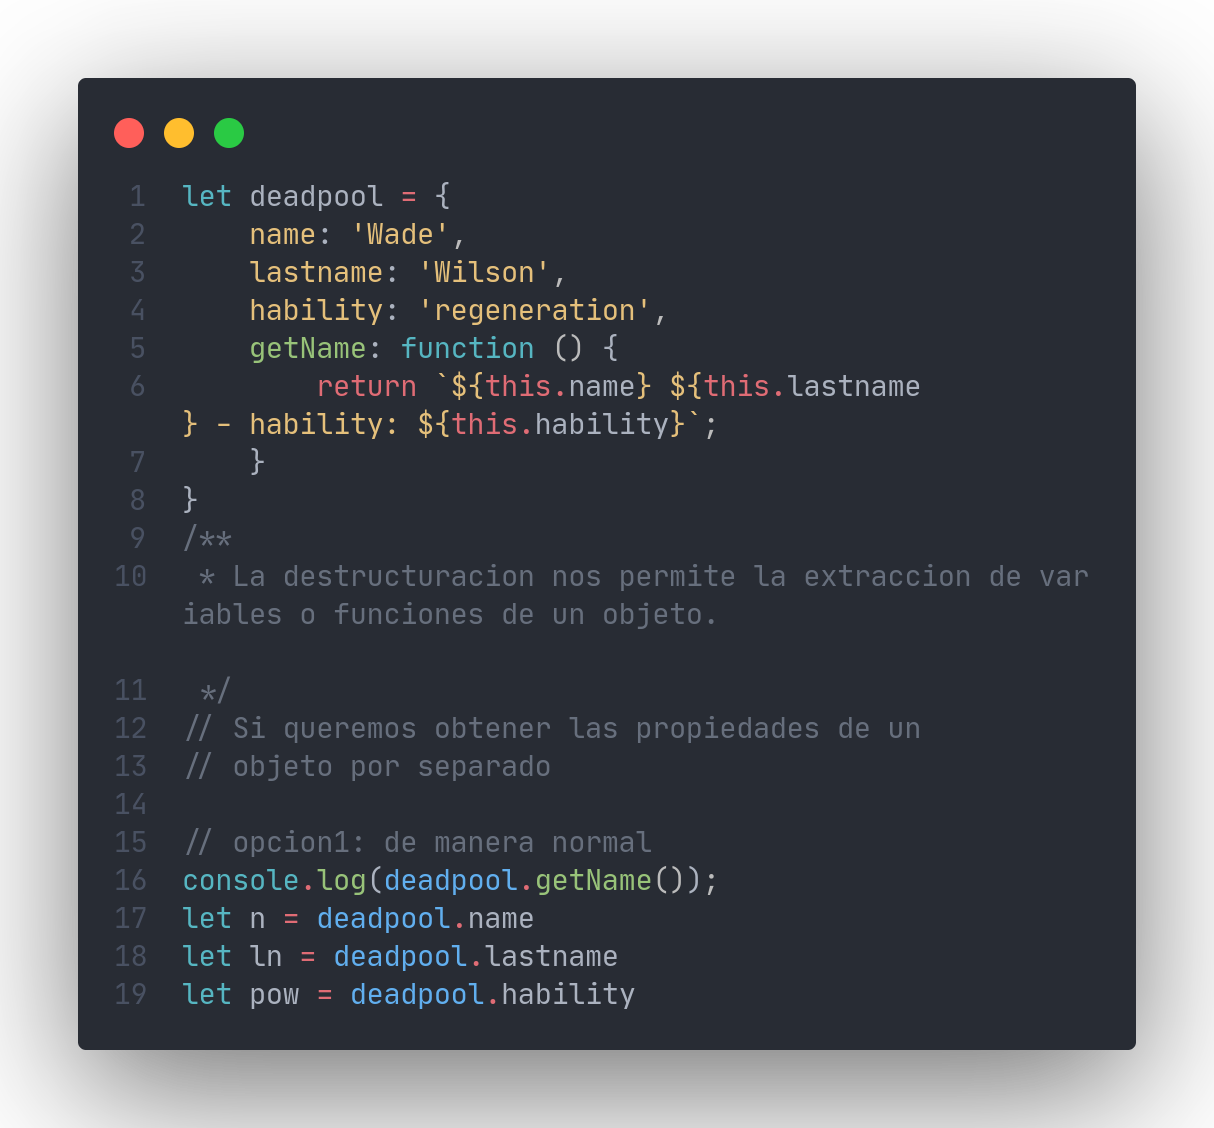
\includegraphics[scale=0.25]{assets/images/destructuracion-1.png}
	\caption{Extracción de variables sin destructuración	}								    
\end{figure}
		
\begin{figure}[H]
	\centering
	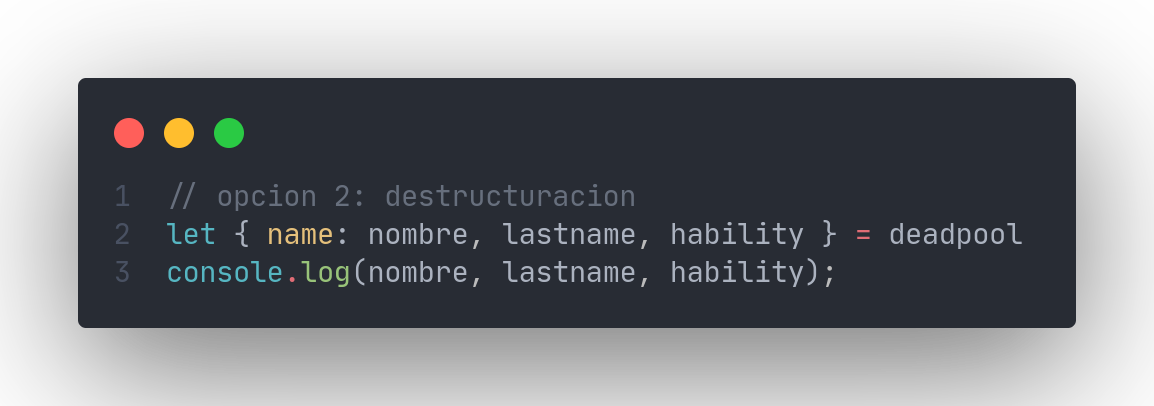
\includegraphics[scale=0.25]{assets/images/destructuracion-2.png}
	\caption{Destructuración}									    
\end{figure}
		
		
\section{Funciones de flecha}

Las funciones de flecha es una nueva forma de escribir funciones, con este método podemos reducir un poco las lineas de código y es un poco mas legible.

\begin{figure}[H]
	\centering
	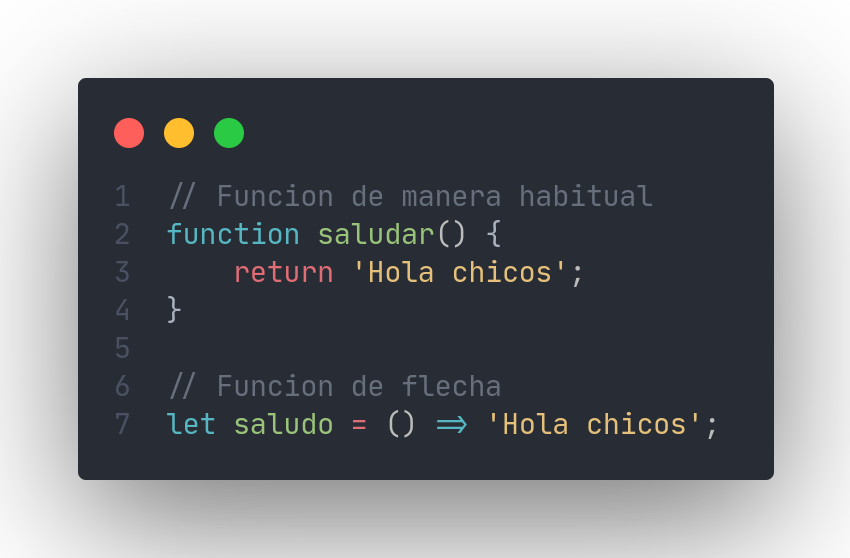
\includegraphics[scale=.2]{assets/images/funcion-flecha-1.png}
	\caption{Funciones de flecha.}
\end{figure}
		
\subsection{Problemas}

Al usar \lstinline{this} con las funciones de flecha dentro de un objeto literal, hacemos referencia al objeto que engloba a todo el sistema y no al objeto literal en si. En ese caso es mejor usar las funciones de la manera habitual con la palabra reservada \lstinline{function}.

\begin{figure}[H]
	\centering
	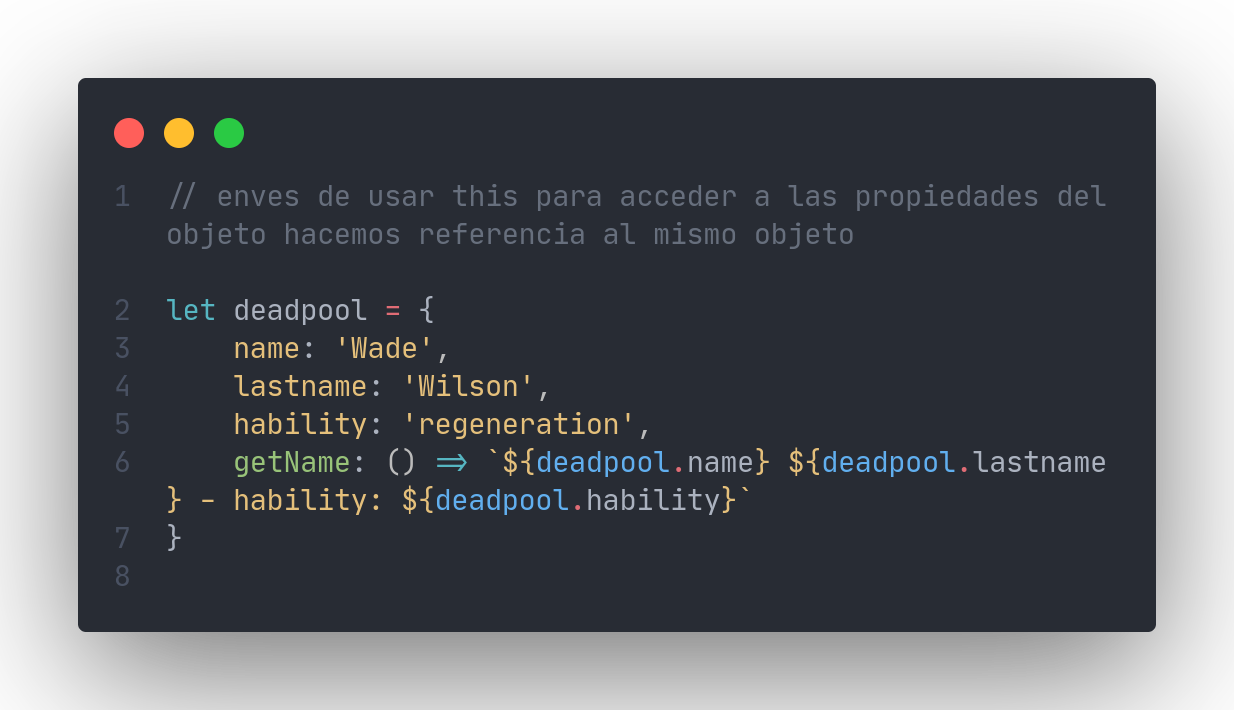
\includegraphics[scale=0.2]{assets/images/funcion-flecha-2.png}
	\caption{Referencia al objeto envés de usar this.}
\end{figure}
		
\section{Callbacks}

La asincronía de javascript trae muchos beneficos, pero tambien un par de problemas y es que los procesos que queremos ejecutar de manera sincrónica es un poco dificil. Para solucionar esto tenemos los callbacks que simplemente es ejecutar una funcion dentro de otra.

\begin{figure}[H]
	\centering
	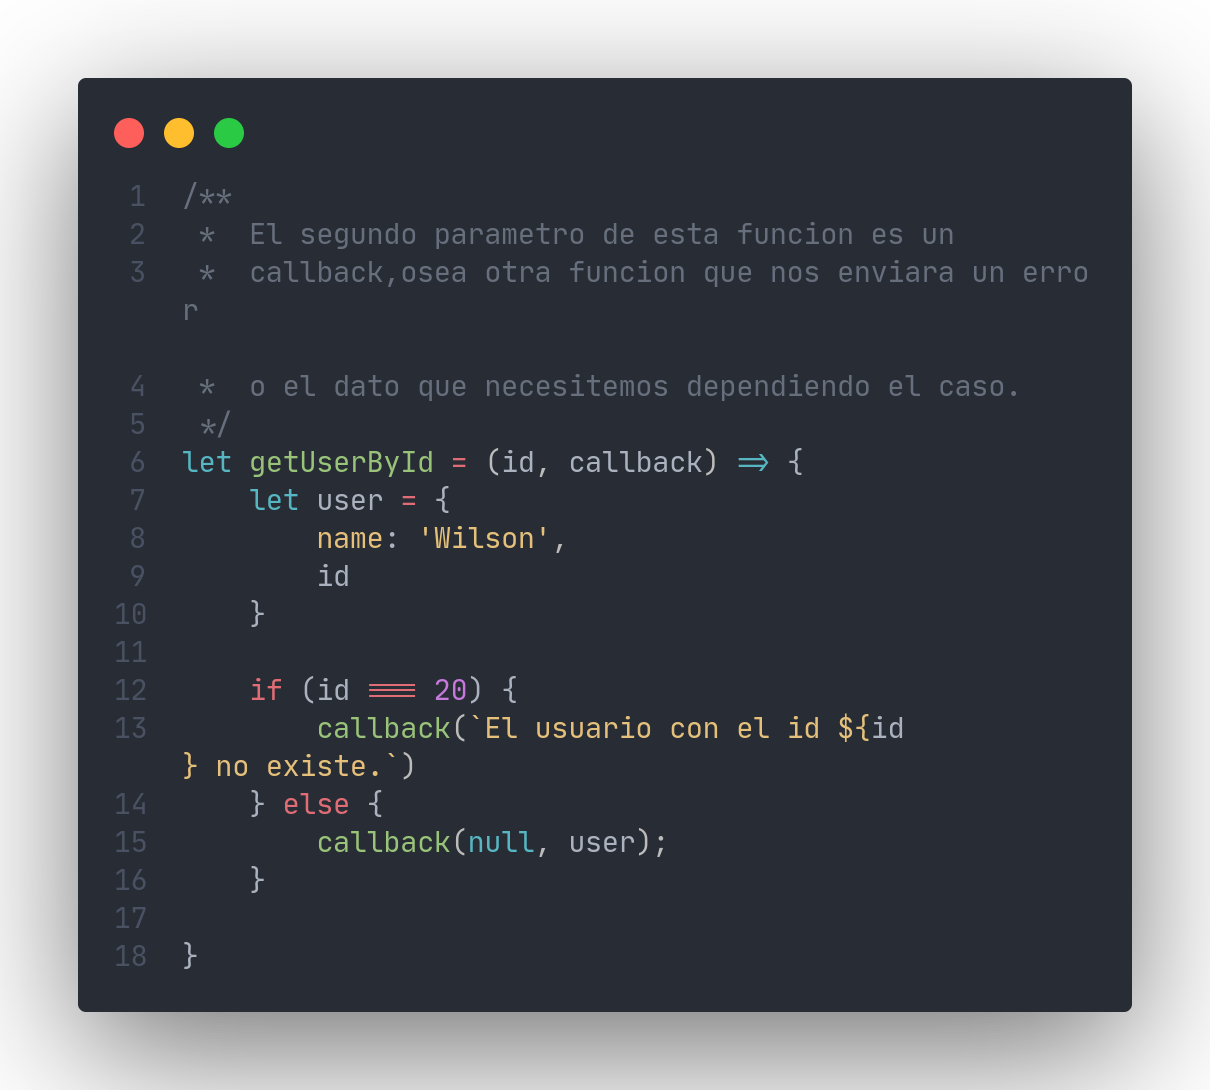
\includegraphics[scale=0.3]{assets/images/callbacks-1.png}
	\caption{Definicion de un callback.}
\end{figure}

Para usar el callback lo usamos igual que una funcion, solo que en el argumento de callback enves de enviar una variable enviamos una funcion que se encargara de manejar los datos enviados, en este caso el usuario.

\begin{figure}[H]
	\centering
	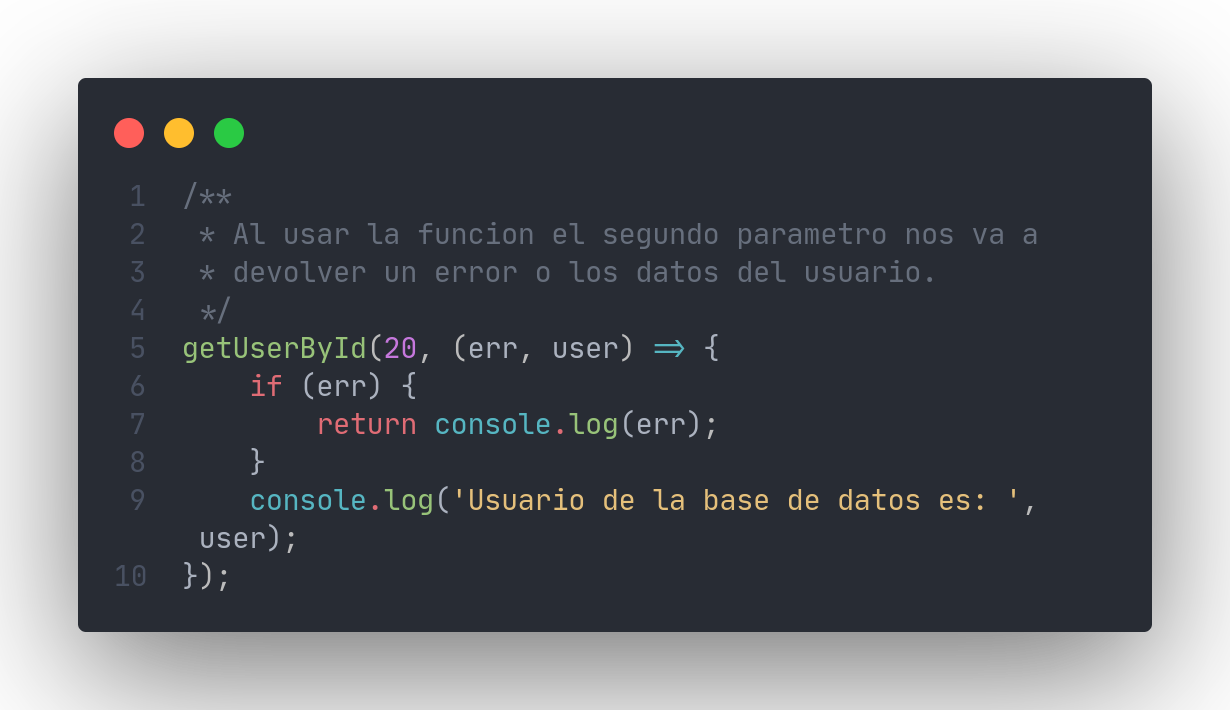
\includegraphics[scale=0.2]{assets/images/callbacks-2.png}
	\caption{Uso del callback}
\end{figure}

\subsection{Problemas}
Los callbacks tienen un problema y es que cuando queremos ejecutar varias acciones de manera sincrónica, el codigo empieza a verse poco legible y se empieza a formar una especie de cascada.

\begin{figure}[H]
	\centering
	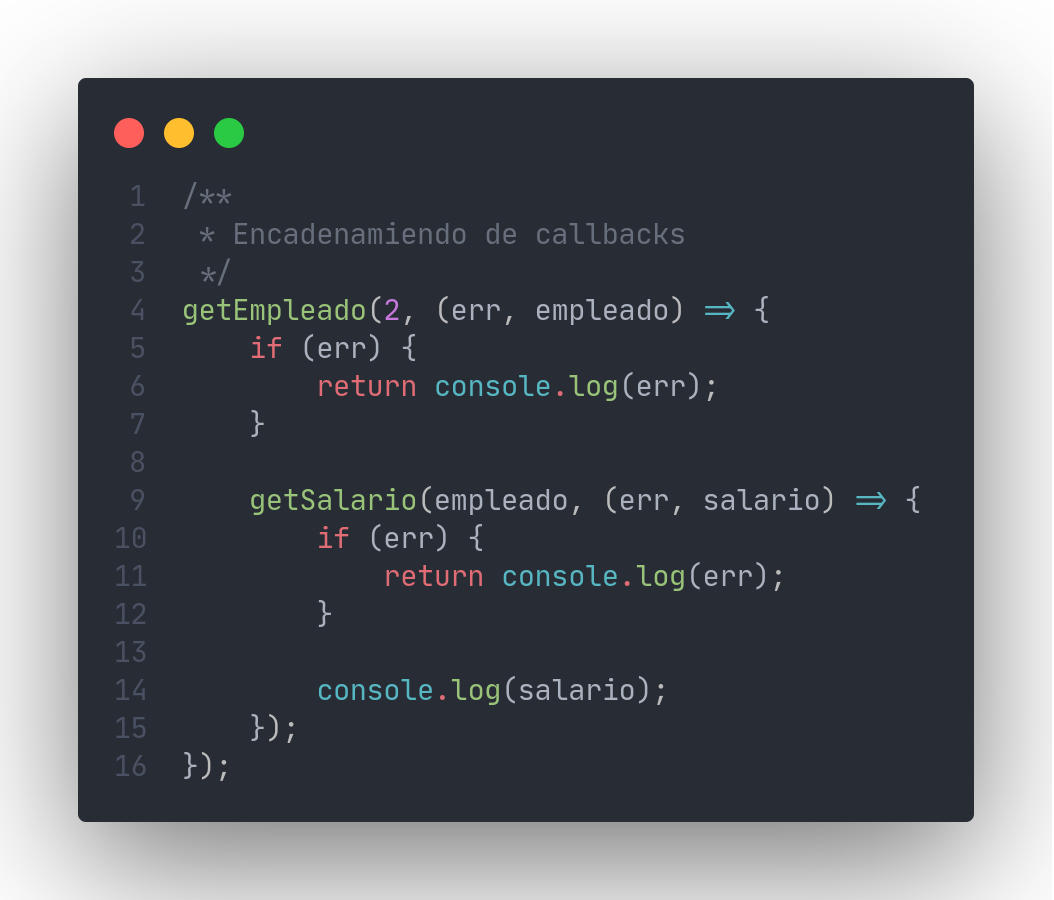
\includegraphics[scale=0.25]{assets/images/callbacks-3.png}
	\caption{Callbacks en cadena}
\end{figure}

\section{Promesas}

Las promesas en javascript son una alternativa a los callbacks. Nos permitesn hacer procesos asíncronos de manera síncrona. El cambio radica es que ya no vamos a recibir un callback en la funcion, solo recibirá el parametro normal. La funcion devolverá una nueva promesa y para devolver el resultado de la promesa usamos \lstinline{resolve()}, en caso de que queramos enviar un error usamos \lstinline{reject()}.

\begin{figure}[H]
	\centering
	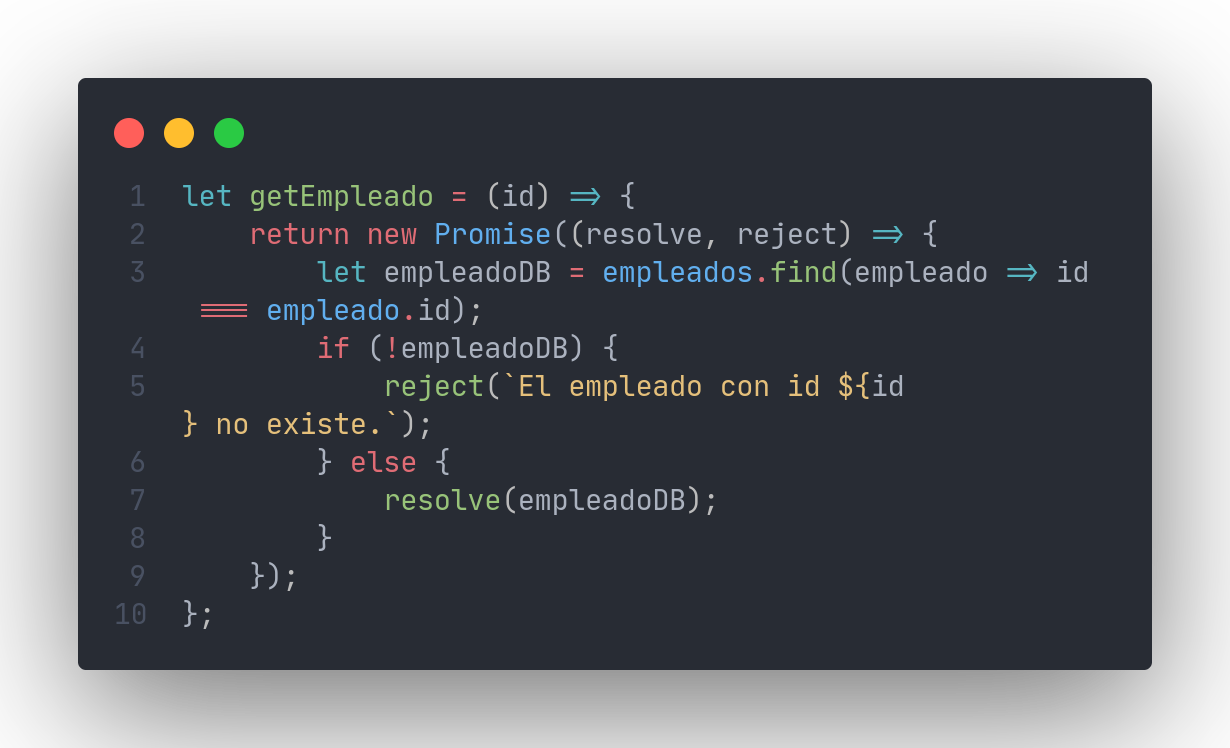
\includegraphics[scale=.3]{assets/images/promesas-1.png}
	\caption{Ejemplo de promesas}
\end{figure}

Para ejecutar promsas tenemos el método \lstinline{.then()} que recie 2 callbacks, el primero se encarga de manejar la promesa resuelta o el \lstinline{resolve} y el segundo se encarga de manejar cuando se ejecuta el \lstinline{reject} del la promesa.

\begin{figure}[H]
	\centering
	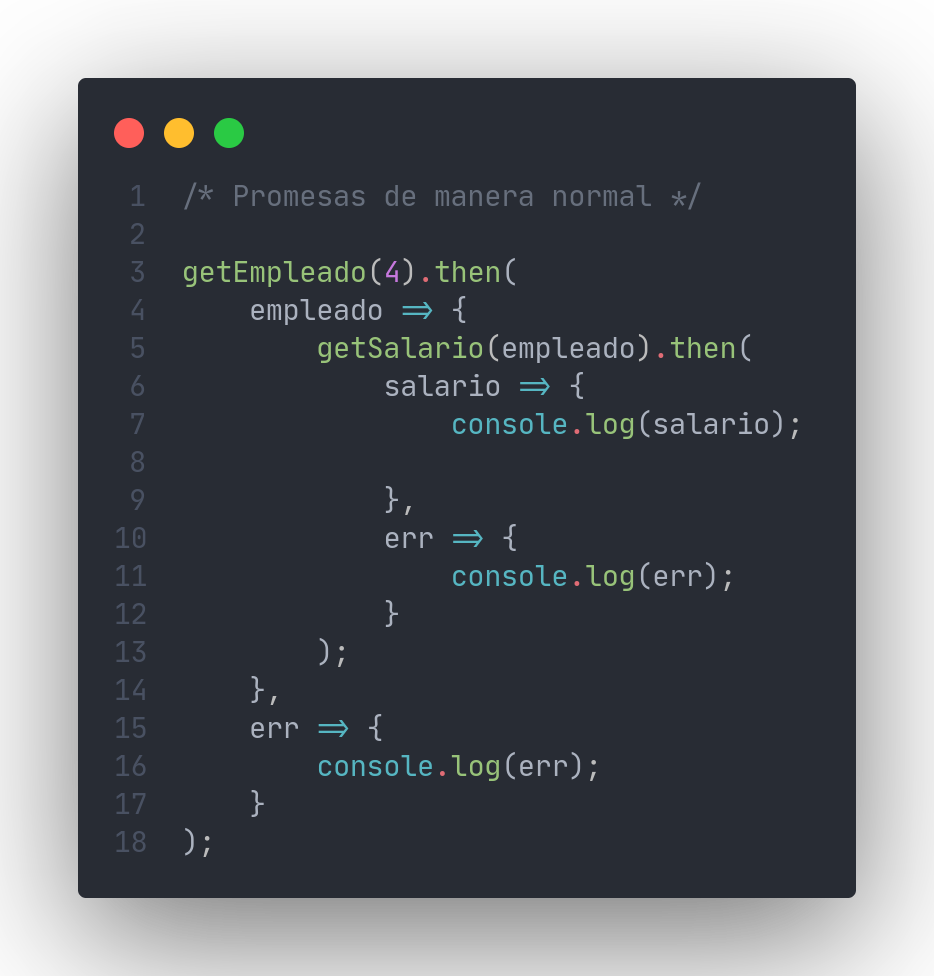
\includegraphics[scale=0.2]{assets/images/promesas-2.png}
	\caption{Ejecucion de varias promesas.}
\end{figure}

Tambien tenemos otra forma de manejar las promesas, y es que las podemos encadenar lo que nos permite ahorrar algunas lineas de código. Envés de ejecutar una promesa dentro de otra lo que hacemos es devolver la ejecucion de otra promesa, asi se van encadenando y para manejar errores que se produzcan en cualquiera de las promesas usamos el metodo \lstinline{.catch()} una sola vez.

\begin{figure}[H]
	\centering
	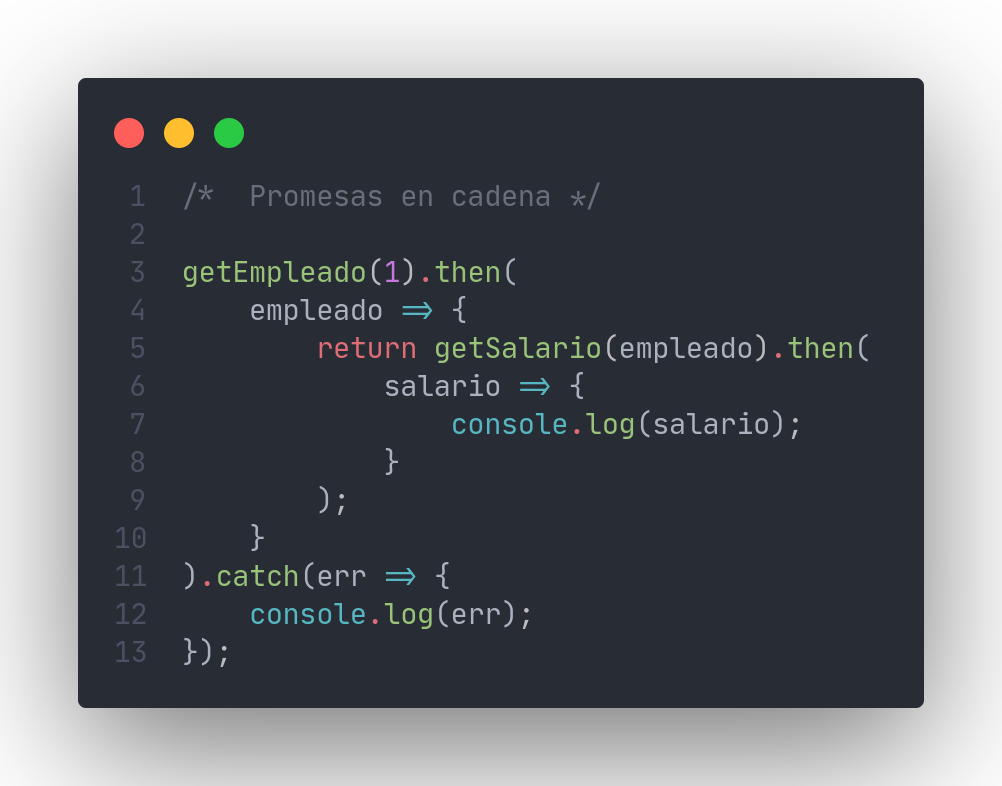
\includegraphics[scale=.24]{assets/images/promesas-3.png}
	\caption{Encadenamiento de promesas.}
\end{figure}
				
\section{Async - Await}

Las funciones \lstinline{async} y \lstinline{await} nos permiten manejar las promesas de una manera mucho mejor.

Async nos permite definir una funcion asíncrona que como resultado nos va a devolver una promesa que podrá ser manejada como tal. El \lstinline{resolve} de esta funcion sera igual a hacer un simple \lstinline{return} y en caso de querer hacer un \lstinline{reject} lanzamos un error con \lstinline{throw new Error()}.

\begin{figure}[H]
	\centering
	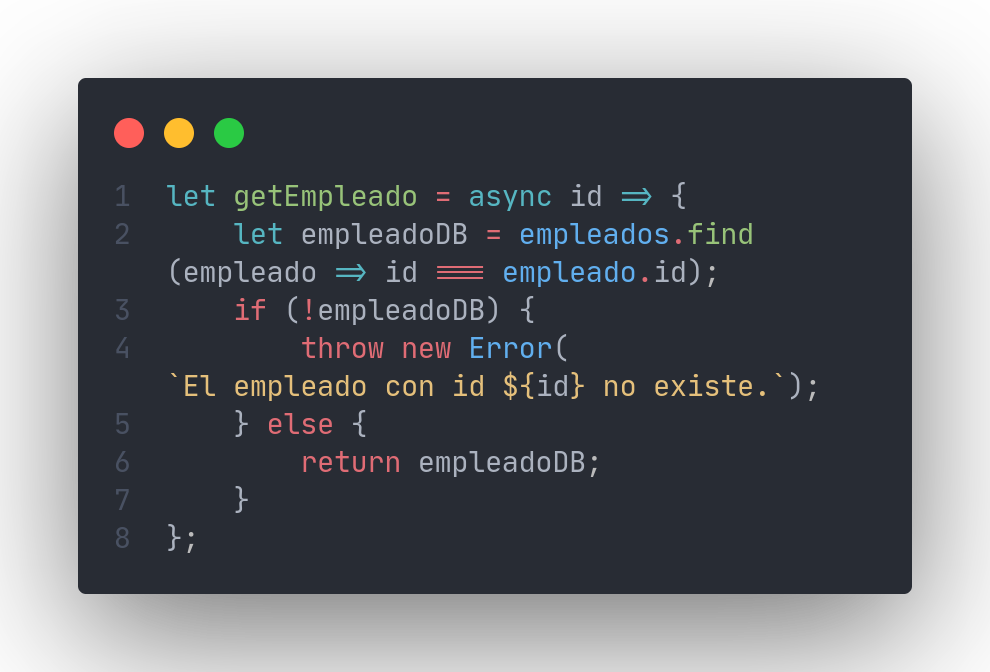
\includegraphics[scale=.3]{assets/images/async.png}
	\caption{Ejemplo de async functions}
\end{figure}

Para manejar varias funciones async que simulen un proceso síncrono podemos usar el \lstinline{await} que espera a que la promesa sea resuelta y nos devuelve el valor de esa promesa que la podemos guardar en una variable. 
Este operador \lstinline{await} solo puede ser usado dentro de una funcion async.

\begin{figure}[H]
	\centering
	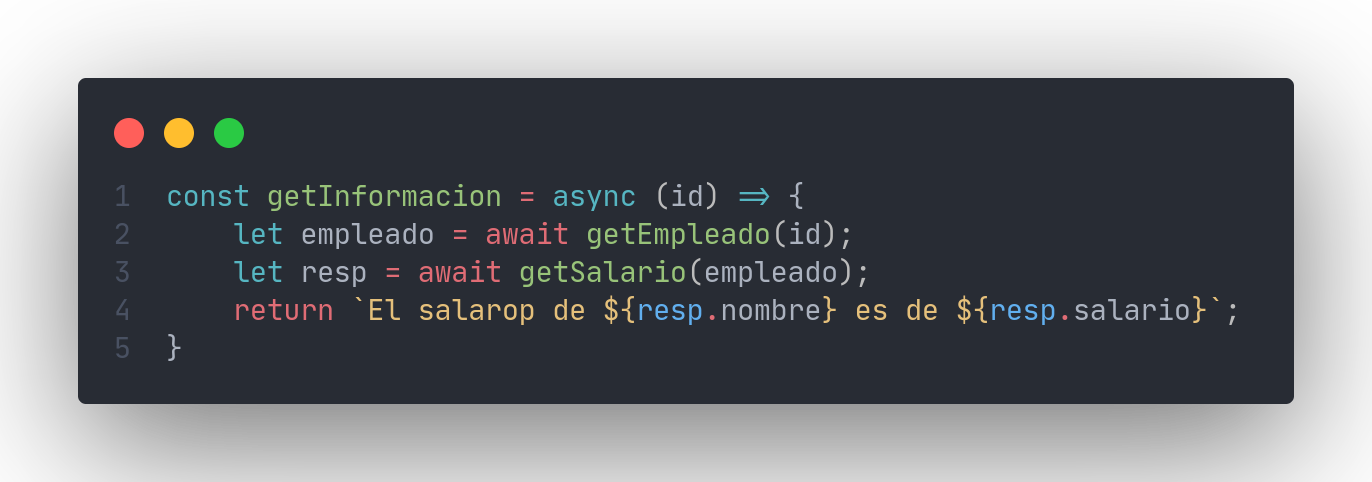
\includegraphics[scale=.28]{assets/images/await.png}
	\caption{Ejemplo de await}
\end{figure}

En caso de que suceda un error podemos manejarlo de manera que fuera una promesa con el metodo \lstinline{.catch()}.

\begin{figure}[H]
	\centering
	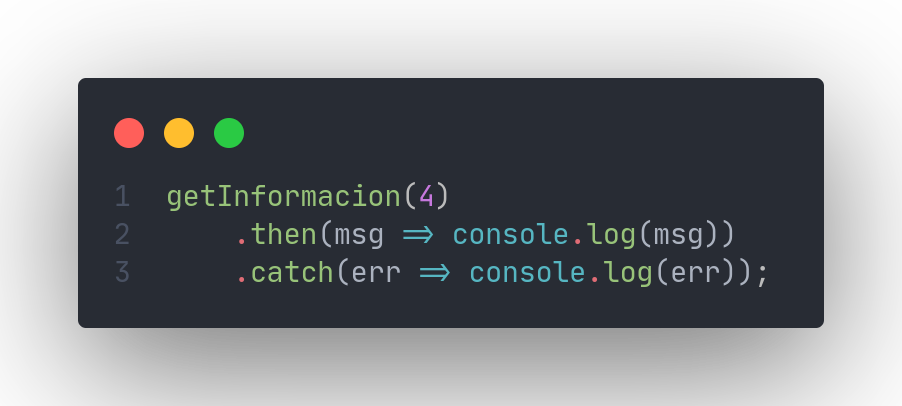
\includegraphics[scale=.3]{assets/images/await-2.png}
	\caption{Capturando error en async function}
\end{figure}
                
\section{Repositorio de la práctica}

El código de la práctica se encuentra en el siguiente enlace: 

\href{https://github.com/WilsonAG/plataformas-web/tree/master/node/02-fundamentos}{repositorio de github.}

\end{document}